% =====================================================================
% Mục 4 — Kết quả thực nghiệm  (BẢN TIẾNG VIỆT)
%
% Bản dịch đối ứng 1-1 với sections/04_results.tex. MỌI CON SỐ phải giống
% bản tiếng Anh; khi sửa số liệu, sửa cả hai bản rồi chạy lại script kiểm tra.
%
% XUẤT XỨ. Mọi phát biểu định lượng trong mục này đều trỏ tới một bảng hoặc
% một hình, và mọi bảng/hình đều trỏ về registry bất biến dưới đây.
%
%   Registry   : docs/reports/experiments/phase_1b/final_b_new_recomputed/
%                20260819T043733Z/
%   Tạo lúc    : 2026-08-19T04:37:33.586402+00:00
%   Git commit : 75df6c061eca5a3d63cfac706d1b6e256e404342
%   Split      : task-B-group-split:359be7f5379818d4
%
% QUY TẮC BÁO CÁO. Độ phân tán luôn là ĐỘ LỆCH CHUẨN trên ba seed chính.
% Nó không bao giờ là ước lượng khoảng, và không gắn bất kỳ khẳng định nào
% về độ tin cậy thống kê cho các chênh lệch trong mục này.
%
% DẤU THẬP PHÂN: giữ dấu chấm như bản tiếng Anh, để phép kiểm tra trùng khớp
% tập con số giữa hai bản còn hiệu lực.
% =====================================================================

\section{Kết quả thực nghiệm}
\label{vi:sec:results}

\subsection{Thiết lập thực nghiệm}
\label{vi:sec:results:setup}

\paragraph{Dữ liệu.} Phân hoạch Task~B gồm 17 loài cây lá kim, chia
3{,}365 / 903 / 532 ảnh cho train / validation / test. Các con số này lấy từ
manifest phân chia đi kèm registry đánh giá nêu ở đầu mục, và số ảnh test của
từng loài được liệt kê ở Bảng~\ref{tab:perspecies_full}. Ba loài khác có trong
bộ sưu tập gốc (\textit{Calocedrus} sp., \textit{Cupressus funebris},
\textit{Pinus} sp.) bị loại vì chỉ định danh được tới cấp chi. Phân hoạch được
gom theo \emph{khóa nguồn} (origin key): các ảnh cùng một khóa nguồn đều nằm
trong cùng một tập, thay vì chia lẻ từng ảnh. Khóa nguồn được suy ra từ tên
tệp và nhằm đại diện cho mẫu gỗ vật lý, sao cho ảnh test đến từ những mẫu vật
mô hình chưa từng thấy, chứ không phải từ các lát cắt khác của mẫu đã quen.
Việc khóa này có tương ứng một-một với mẫu vật vật lý hay không thì \textbf{chưa
được chứng minh}; Mục~\ref{vi:sec:discussion:originkey} trình bày rõ cách gom
này bảo đảm được gì và không bảo đảm được gì.

\paragraph{Phân họ.} Các loài được nhóm vào năm họ (Araucariaceae,
Cupressaceae, Pinaceae, Podocarpaceae và Taxaceae) theo phân loại học cây lá
kim được chấp nhận, tức \textit{Araucaria araucana} thuộc Araucariaceae. Điều
này khác với sơ đồ bốn họ của nhiệm vụ cấp họ trong dự án, vốn gộp loài đó vào
Pinaceae. Việc phân họ chỉ ảnh hưởng đến cách nhóm kết quả khi trình bày. Nó không
tham gia vào huấn luyện hay đánh giá, và mọi con số theo từng loài đều
không đổi vì lựa chọn này. Các tỷ lệ lỗi ở cấp họ trong mục này đều được tính
theo sơ đồ năm họ.

\paragraph{Cấu hình huấn luyện.} Cả năm backbone đều khởi tạo từ trọng số
ImageNet và tinh chỉnh trong 50 epoch với lịch cosine, tốc độ học phần đầu
$1\times10^{-4}$, tốc độ học phần thân $1\times10^{-5}$, weight decay
$1\times10^{-4}$, label smoothing 0.1 và huấn luyện độ chính xác hỗn hợp. Các
thiết lập này giống nhau trên cả 30 lần chạy đã đăng ký. Kích thước lô là
tham số duy nhất thay đổi, và nó thay đổi \emph{theo backbone} chứ không theo
thí nghiệm: 64 cho ResNet-50 và MobileNetV3-Large, 32 cho EfficientNet-B3,
ConvNeXt-Tiny và Swin-Tiny, giữ cố định cho từng backbone qua cả các lần chạy
chính lẫn ba ablation. Do đó phép so sánh giữa một ablation và đường cơ sở của
nó là so sánh \emph{trong cùng backbone} và chỉ đổi một biến; còn so sánh
\emph{giữa các backbone} mang thêm kích thước lô như một khác biệt chưa được
kiểm soát.

\paragraph{Seed và đánh giá.} Cấu hình chính được huấn luyện với ba seed
(42, 123, 456), cho 15 lần chạy chính. Mỗi ablation chỉ huấn luyện với seed 42,
cho 5 lần chạy mỗi ablation. Đánh giá dùng FP16 autocast, phép nhân ma trận
TF32 và bộ nhớ channels-last trên NVIDIA GeForce RTX 4090 với PyTorch
2.11.0+cu128, toàn bộ tập dữ liệu nằm sẵn trên GPU nên kích thước lô không ảnh
hưởng kết quả.

\subsection{Benchmark chính}
\label{vi:sec:results:benchmark}

Bảng~\ref{tab:task_b} báo cáo độ chính xác test và macro-F1 cho năm kiến trúc,
dưới dạng trung bình và độ lệch chuẩn trên ba seed chính.

% Table: Task B main benchmark (species-level, 17 classes)
% AUTO-GENERATED bang scripts/person3/make_result_tables.py -- khong sua tay
% Source file      : docs/reports/experiments/phase_1b/final_b_new_recomputed/20260819T043733Z/main_test_summary.csv
% Registry created : 2026-08-19T04:37:33.586402+00:00
% Source run ids   : 15 runs
%   taskB17__main__seed_123__convnext_tiny
%   taskB17__main__seed_123__efficientnet_b3
%   taskB17__main__seed_123__mobilenetv3_large
%   taskB17__main__seed_123__resnet50
%   taskB17__main__seed_123__swin_tiny
%   taskB17__main__seed_42__convnext_tiny
%   taskB17__main__seed_42__efficientnet_b3
%   taskB17__main__seed_42__mobilenetv3_large
%   taskB17__main__seed_42__resnet50
%   taskB17__main__seed_42__swin_tiny
%   taskB17__main__seed_456__convnext_tiny
%   taskB17__main__seed_456__efficientnet_b3
%   taskB17__main__seed_456__mobilenetv3_large
%   taskB17__main__seed_456__resnet50
%   taskB17__main__seed_456__swin_tiny
\begin{table}[!htbp]
\centering
\caption{Hiệu năng phân loại ở cấp loài trên tập test Task~B (17 loài, 532 ảnh, phân hoạch gom theo khóa nguồn sao cho các ảnh cùng một khóa nguồn nằm trong cùng một tập). Giá trị là trung bình $\pm$ độ lệch chuẩn trên 3 seed huấn luyện (42, 123, 456); độ phân tán được báo cáo là độ lệch chuẩn trên ba lần chạy, không phải ước lượng khoảng. Giá trị tốt nhất mỗi cột in đậm.}
\label{tab:task_b}
\begin{tabular}{lcc}
\toprule
\textbf{Kiến trúc} & \textbf{Độ chính xác Top-1 (\%)} & \textbf{Macro-F1 (\%)} \\
\midrule
ResNet-50         & $92.356 \pm 1.022$ & $92.569 \pm 0.982$ \\
EfficientNet-B3   & $97.807 \pm 0.319$ & $97.844 \pm 0.322$ \\
MobileNetV3-Large & $98.371 \pm 0.319$ & $98.448 \pm 0.345$ \\
ConvNeXt-Tiny     & $\mathbf{99.561 \pm 0.354}$ & $\mathbf{99.596 \pm 0.326}$ \\
Swin-Tiny         & $99.123 \pm 0.581$ & $99.196 \pm 0.533$ \\
\bottomrule
\end{tabular}
\end{table}


Hai backbone hiện đại dẫn đầu. ConvNeXt-Tiny đạt
$99.561 \pm 0.354$\,\% độ chính xác và $99.596 \pm 0.326$\,\% macro-F1,
trên Swin-Tiny với $99.123 \pm 0.581$\,\% và $99.196 \pm 0.533$\,\%.
MobileNetV3-Large theo sau với $98.371 \pm 0.319$\,\% dù là mô hình nhỏ nhất
trong nhóm so sánh, còn EfficientNet-B3 đạt $97.807 \pm 0.319$\,\%. ResNet-50
xếp cuối với khoảng cách rõ ràng, $92.356 \pm 1.022$\,\% độ chính xác và
$92.569 \pm 0.982$\,\% macro-F1, thấp hơn mô hình dẫn đầu khoảng bảy điểm
và có độ phân tán giữa các seed lớn nhất trong năm.

Có hai đặc điểm của độ phân tán cần nêu trước khi đọc thứ hạng quá chắc chắn.
Thứ nhất, khoảng cách giữa ConvNeXt-Tiny, Swin-Tiny và MobileNetV3-Large cùng
bậc độ lớn với chính độ lệch chuẩn giữa các seed, nên thứ tự giữa ba mô hình
này dựa trên những chênh lệch mà một bộ seed khác hoàn toàn có thể đảo lại.
Thứ hai, khoảng cách của ResNet-50 so với phần còn lại gấp nhiều lần độ lệch
chuẩn của chính nó, và đây là thứ tự duy nhất trong bảng không phụ thuộc vào
cảnh báo trên.

Độ chính xác và macro-F1 bám sát nhau ở mọi backbone, điều này hợp lý vì tập
test gần cân bằng, với số ảnh mỗi loài dao động từ 24 đến 39
(Bảng~\ref{tab:perspecies_full}). Không backbone nào đổi độ chính xác bằng
cách bỏ qua một lớp nhỏ.

\subsection{Phân tích theo loài và ma trận nhầm lẫn}
\label{vi:sec:results:perspecies}

\paragraph{Chọn mô hình.} Ma trận nhầm lẫn chỉ báo cáo cho một kiến trúc, chọn
theo tiêu chí được cố định \emph{trước khi} xem cấu trúc nhầm lẫn: backbone có
macro-F1 trung bình cao nhất trên ba seed chính, tức ConvNeXt-Tiny
(Bảng~\ref{tab:task_b}). Phương án báo cáo lần chạy đơn lẻ có điểm cao nhất đã
bị loại, và thực tế nó cũng vô định ở đây: seed 42 và seed 123 hòa nhau đúng
99.812\,\% độ chính xác mà không có quy tắc phá hòa nào được nêu.

\paragraph{Cách gộp.} Hình~\ref{fig:confusion} cộng theo từng phần tử ba ma
trận đếm $17\times17$ của ba seed, cho $532\times3 = 1{,}596$ dự đoán. Mỗi
seed đóng góp như nhau, và việc chuẩn hóa theo hàng chia cho tổng hàng của
các count đã cộng. Ba ma trận riêng từng seed được công bố kèm bản gộp để có
thể kiểm tra lại phép cộng.

\paragraph{Kết quả.} ConvNeXt-Tiny mắc 7 lỗi trên 1{,}596 dự đoán, và cả 7 đều
là cùng một nhầm lẫn: \textit{Pinus krempfii} bị dự đoán thành
\textit{Pinus dalatensis}. Ngoài ra ma trận hoàn toàn là đường chéo. Cả hai
loài đều thuộc Pinaceae, nên không có lỗi nào vượt qua ranh giới họ.

% Figure: 17x17 confusion matrix, ConvNeXt-Tiny, counts summed over 3 seeds
% Source     : docs/reports/experiments/phase_1b/final_b_new_recomputed/
%              20260819T043733Z/predictions.csv   (only source of the counts)
% Cross-check: confusion_matrices.npz, exact element-wise after permuting to
%              the family class order -- 0 cells differing on all three seeds
% Artifacts  : artifact/person3/confusion/{confusion_convnext_main.csv,
%              confusion_convnext_main_per_seed.csv, confusion_metadata.json}
% Run ids    : taskB17__main__seed_{42,123,456}__convnext_tiny
\begin{figure}[!htbp]
\centering
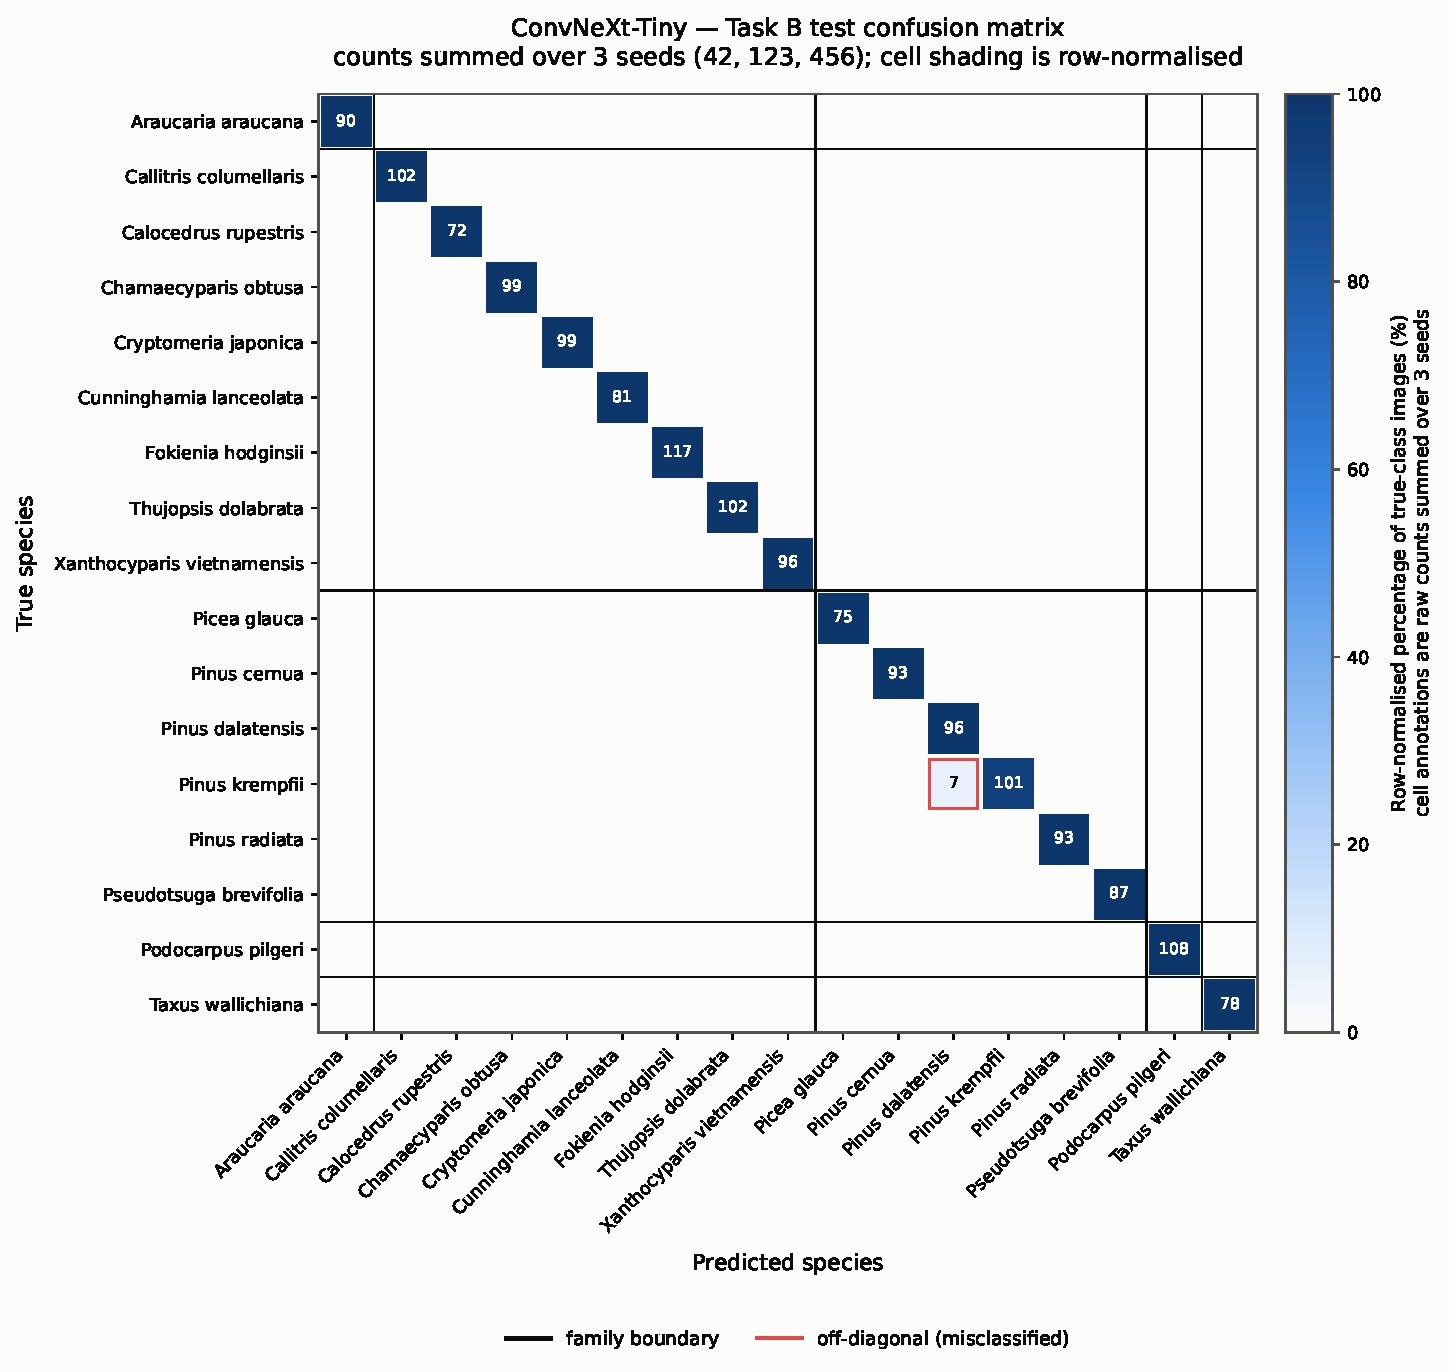
\includegraphics[width=\columnwidth]{artifact/person3/confusion/fig_confusion.pdf}
\caption{Ma trận nhầm lẫn của ConvNeXt-Tiny trên tập test Task~B. Các count được cộng theo từng phần tử qua ba seed chính (42, 123, 456), cho $532\times3 = 1{,}596$ dự đoán; mỗi seed đóng góp như nhau. Màu nền ô là tỷ lệ phần trăm đã chuẩn hóa theo hàng của số ảnh thuộc lớp thật, với mẫu số là tổng hàng của các count đã cộng; số ghi trong mỗi ô là count thô đã cộng. Các loài được sắp theo họ và các đường kẻ đen đánh dấu ranh giới họ. Ô ngoài đường chéo được viền đỏ. ConvNeXt-Tiny được chọn theo tiêu chí cố định trước (macro-F1 trung bình cao nhất trên ba seed ở Bảng~\ref{tab:task_b}), chứ không phải bằng cách xem ma trận này. Ba ma trận riêng từng seed được công bố kèm bản gộp để kiểm tra lại được phép cộng.}
\label{fig:confusion}
\end{figure}


Hình~\ref{fig:perclass} và Bảng~\ref{tab:perspecies_full} cho F1 theo từng loài
ở cả năm backbone. Ba quy luật nổi bật.

% Figure: per-species F1 by architecture (small multiples)
% Source   : docs/reports/experiments/phase_1b/final_b_new_recomputed/
%            20260819T043733Z/per_class_metrics.csv
% Artifacts: artifact/person3/per_class/{perclass_f1_summary.csv,
%            perclass_metadata.json, error_analysis.md}
% Run ids  : 15 (5 backbones x seeds 42/123/456), listed in perclass_metadata.json
\begin{figure}[!htbp]
\centering
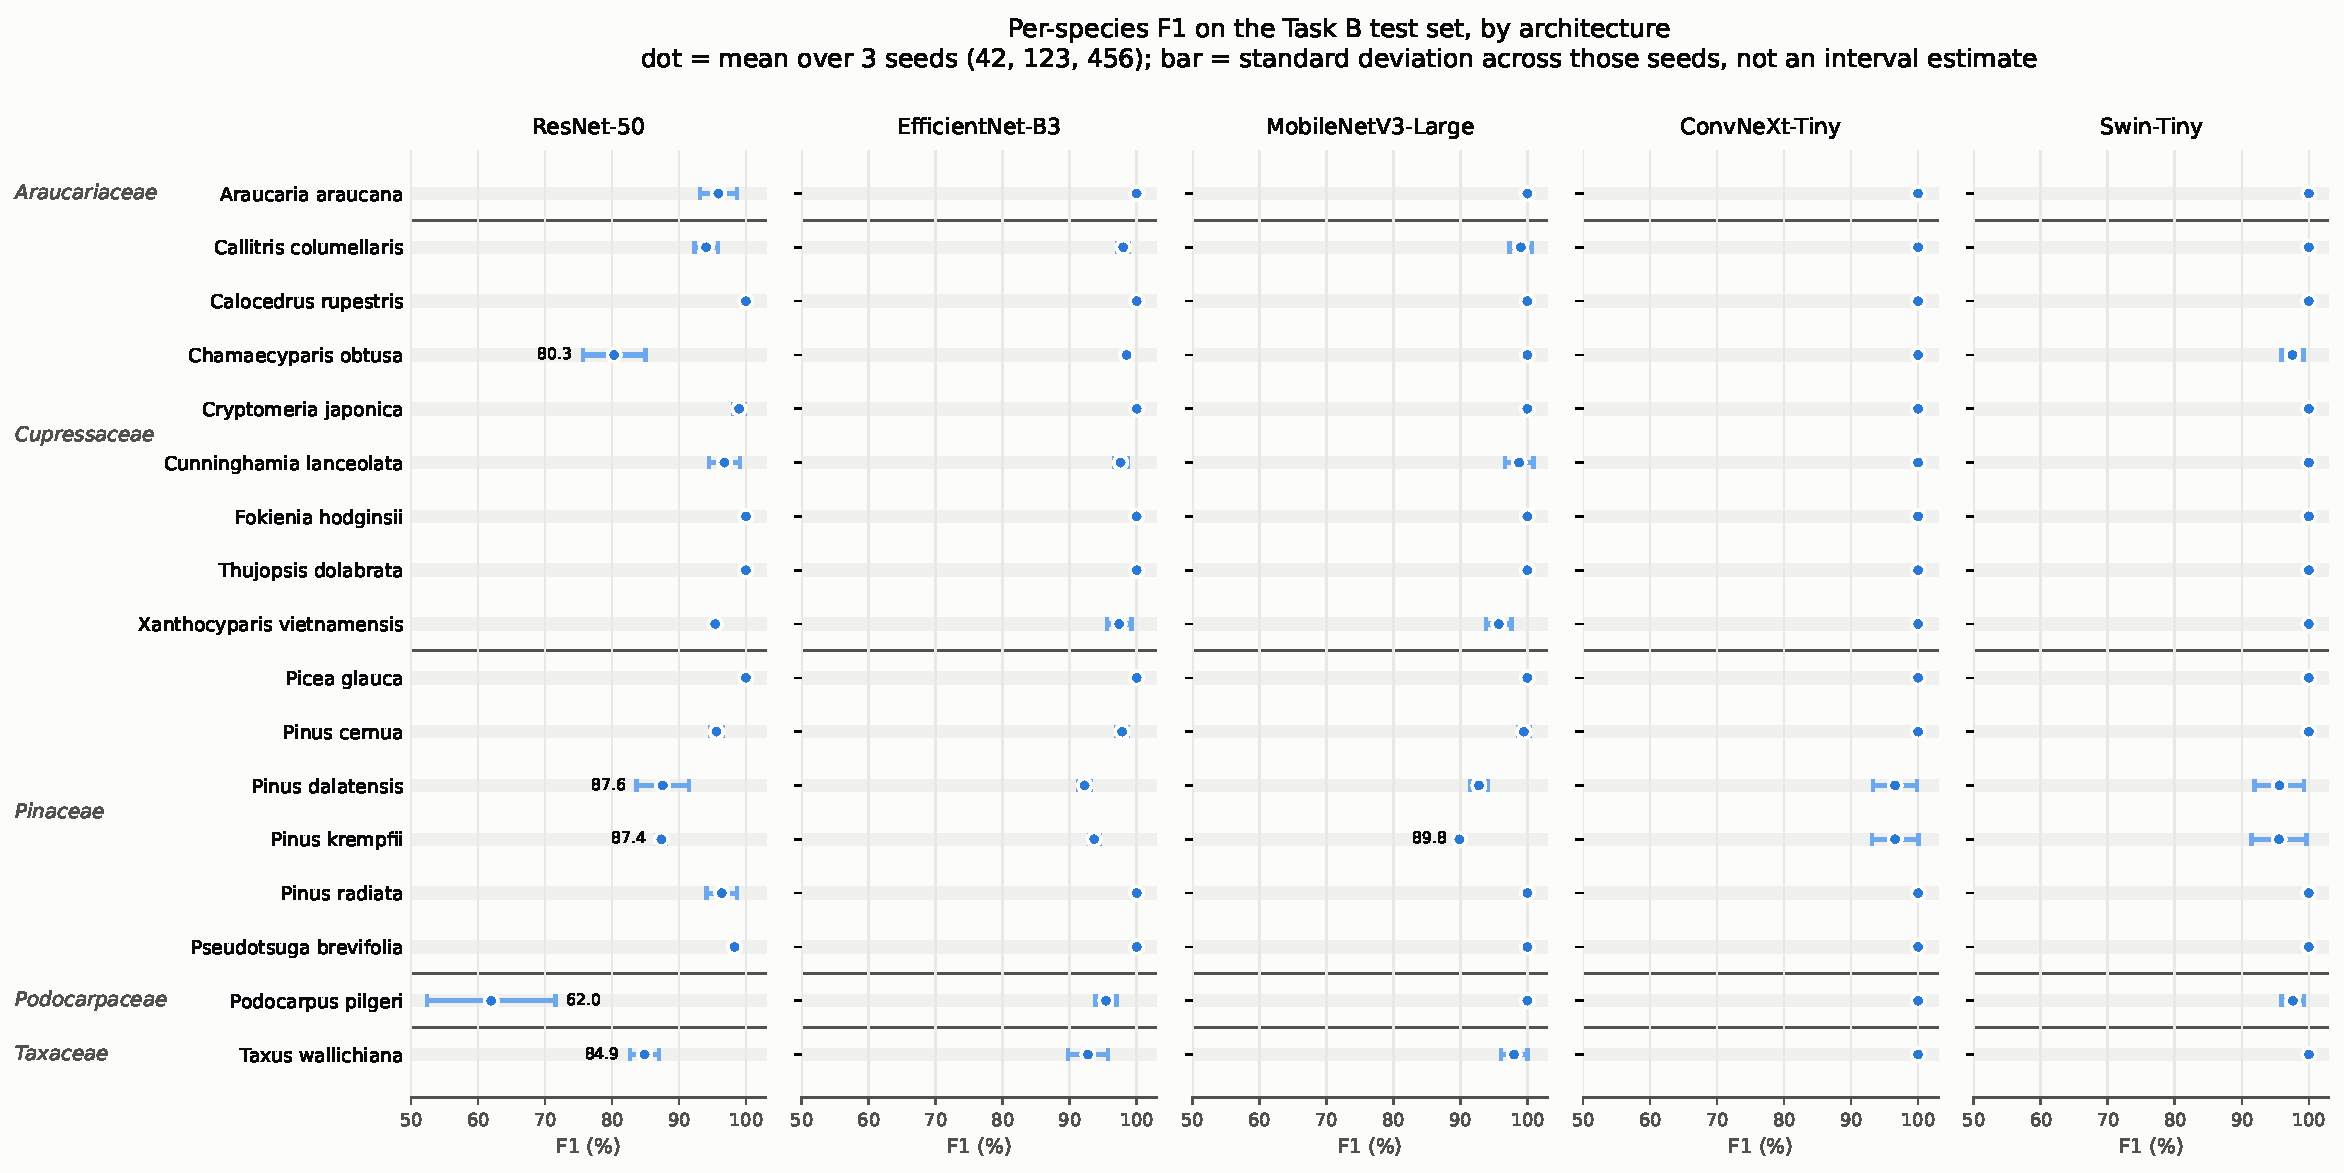
\includegraphics[width=\linewidth]{artifact/person3/per_class/fig_perclass_f1.pdf}
\caption{Điểm F1 theo từng loài trên tập test Task~B, mỗi panel một kiến trúc. Mỗi chấm là trung bình trên ba seed chính (42, 123, 456) và mỗi thanh là độ lệch chuẩn trên các seed đó; thanh này là thước đo phân tán trên ba lần chạy, không phải ước lượng khoảng. Các loài được sắp theo họ, các khối họ tách nhau bằng đường kẻ ngang và được ghi nhãn ở lề trái. Trục ngang mã hóa bằng vị trí nên không bắt đầu từ không; các giá trị dưới 90\,\% được ghi nhãn trực tiếp. Các kiến trúc được tách thành panel riêng thay vì phân biệt bằng màu, để danh tính được mang bởi vị trí và tiêu đề panel.}
\label{fig:perclass}
\end{figure}

% Table: per-species F1, full 17 classes x 5 backbones
% AUTO-GENERATED bang scripts/person3/make_result_tables.py -- khong sua tay
% Source file      : docs/reports/experiments/phase_1b/final_b_new_recomputed/20260819T043733Z/per_class_metrics.csv
% Registry created : 2026-08-19T04:37:33.586402+00:00
% Source run ids   : 15 runs
%   taskB17__main__seed_123__convnext_tiny
%   taskB17__main__seed_123__efficientnet_b3
%   taskB17__main__seed_123__mobilenetv3_large
%   taskB17__main__seed_123__resnet50
%   taskB17__main__seed_123__swin_tiny
%   taskB17__main__seed_42__convnext_tiny
%   taskB17__main__seed_42__efficientnet_b3
%   taskB17__main__seed_42__mobilenetv3_large
%   taskB17__main__seed_42__resnet50
%   taskB17__main__seed_42__swin_tiny
%   taskB17__main__seed_456__convnext_tiny
%   taskB17__main__seed_456__efficientnet_b3
%   taskB17__main__seed_456__mobilenetv3_large
%   taskB17__main__seed_456__resnet50
%   taskB17__main__seed_456__swin_tiny
\begin{table}[!htbp]
\centering
\footnotesize
\setlength{\tabcolsep}{3pt}
\caption{Điểm F1 theo từng loài (\%) trên tập test Task~B (17 loài, 532 ảnh), cho từng backbone. Giá trị là trung bình $\pm$ độ lệch chuẩn trên 3 seed huấn luyện chính (42, 123, 456); độ phân tán là độ lệch chuẩn trên ba lần chạy, không phải ước lượng khoảng. Các loài được nhóm theo họ. $n$ là số ảnh test của mỗi loài.}
\label{tab:perspecies_full}
\resizebox{\linewidth}{!}{%
\begin{tabular}{lrccccc}
\toprule
\textbf{Loài} & $n$ & \textbf{ResNet-50} & \textbf{EfficientNet-B3} & \textbf{MobileNetV3-Large} & \textbf{ConvNeXt-Tiny} & \textbf{Swin-Tiny} \\
\midrule
\multicolumn{7}{l}{\textit{Araucariaceae}} \\
\quad \textit{Araucaria araucana} & 30 & $95.905 \pm 2.781$ & $100.000 \pm 0.000$ & $100.000 \pm 0.000$ & $100.000 \pm 0.000$ & $100.000 \pm 0.000$ \\
\midrule
\multicolumn{7}{l}{\textit{Cupressaceae}} \\
\quad \textit{Callitris columellaris} & 34 & $94.067 \pm 1.734$ & $97.995 \pm 0.888$ & $99.020 \pm 1.698$ & $100.000 \pm 0.000$ & $100.000 \pm 0.000$ \\
\quad \textit{Calocedrus rupestris} & 24 & $100.000 \pm 0.000$ & $100.000 \pm 0.000$ & $100.000 \pm 0.000$ & $100.000 \pm 0.000$ & $100.000 \pm 0.000$ \\
\quad \textit{Chamaecyparis obtusa} & 33 & $80.336 \pm 4.658$ & $98.492 \pm 0.027$ & $100.000 \pm 0.000$ & $100.000 \pm 0.000$ & $97.556 \pm 1.649$ \\
\quad \textit{Cryptomeria japonica} & 33 & $98.974 \pm 0.888$ & $100.000 \pm 0.000$ & $100.000 \pm 0.000$ & $100.000 \pm 0.000$ & $100.000 \pm 0.000$ \\
\quad \textit{Cunninghamia lanceolata} & 27 & $96.781 \pm 2.307$ & $97.597 \pm 1.012$ & $98.765 \pm 2.138$ & $100.000 \pm 0.000$ & $100.000 \pm 0.000$ \\
\quad \textit{Fokienia hodginsii} & 39 & $100.000 \pm 0.000$ & $100.000 \pm 0.000$ & $100.000 \pm 0.000$ & $100.000 \pm 0.000$ & $100.000 \pm 0.000$ \\
\quad \textit{Thujopsis dolabrata} & 34 & $100.000 \pm 0.000$ & $100.000 \pm 0.000$ & $100.000 \pm 0.000$ & $100.000 \pm 0.000$ & $100.000 \pm 0.000$ \\
\quad \textit{Xanthocyparis vietnamensis} & 32 & $95.431 \pm 0.080$ & $97.387 \pm 1.861$ & $95.733 \pm 1.892$ & $100.000 \pm 0.000$ & $100.000 \pm 0.000$ \\
\midrule
\multicolumn{7}{l}{\textit{Pinaceae}} \\
\quad \textit{Picea glauca} & 25 & $100.000 \pm 0.000$ & $100.000 \pm 0.000$ & $100.000 \pm 0.000$ & $100.000 \pm 0.000$ & $100.000 \pm 0.000$ \\
\quad \textit{Pinus cernua} & 31 & $95.610 \pm 0.915$ & $97.832 \pm 0.916$ & $99.471 \pm 0.916$ & $100.000 \pm 0.000$ & $100.000 \pm 0.000$ \\
\quad \textit{Pinus dalatensis} & 32 & $87.596 \pm 3.913$ & $92.228 \pm 0.911$ & $92.767 \pm 1.345$ & $96.559 \pm 3.295$ & $95.620 \pm 3.706$ \\
\quad \textit{Pinus krempfii} & 36 & $87.383 \pm 0.738$ & $93.663 \pm 0.788$ & $89.849 \pm 0.294$ & $96.573 \pm 3.495$ & $95.548 \pm 4.082$ \\
\quad \textit{Pinus radiata} & 31 & $96.409 \pm 2.273$ & $100.000 \pm 0.000$ & $100.000 \pm 0.000$ & $100.000 \pm 0.000$ & $100.000 \pm 0.000$ \\
\quad \textit{Pseudotsuga brevifolia} & 29 & $98.305 \pm 0.000$ & $100.000 \pm 0.000$ & $100.000 \pm 0.000$ & $100.000 \pm 0.000$ & $100.000 \pm 0.000$ \\
\midrule
\multicolumn{7}{l}{\textit{Podocarpaceae}} \\
\quad \textit{Podocarpus pilgeri} & 36 & $61.994 \pm 9.598$ & $95.420 \pm 1.562$ & $100.000 \pm 0.000$ & $100.000 \pm 0.000$ & $97.612 \pm 1.697$ \\
\midrule
\multicolumn{7}{l}{\textit{Taxaceae}} \\
\quad \textit{Taxus wallichiana} & 26 & $84.891 \pm 2.182$ & $92.732 \pm 2.970$ & $98.013 \pm 2.000$ & $100.000 \pm 0.000$ & $100.000 \pm 0.000$ \\
\bottomrule
\end{tabular}}
\end{table}


\textit{Thứ nhất}, cặp \textit{P.\ krempfii} / \textit{P.\ dalatensis} là
nhầm lẫn duy nhất xuất hiện ở \emph{mọi} kiến trúc: 18, 12, 15, 9 và 7 lần lần
lượt với ResNet-50, EfficientNet-B3, MobileNetV3-Large, Swin-Tiny và
ConvNeXt-Tiny, tổng cộng 61 lần, so với đúng một lần theo chiều ngược lại. Nó
chiếm 61 trong tổng số 204 lỗi của tất cả backbone và seed cộng lại, và không
giảm đi khi năng lực mô hình tăng. Cả hai loài đều thuộc chi \textit{Pinus}
(họ Pinaceae) với số ảnh test tương đương (36 và 32), nên cả mất cân bằng lớp
lẫn ranh giới họ đều không giải thích được hiện tượng này. Hai loài này cũng
mang độ lệch chuẩn giữa các seed lớn nhất trong hai cột mạnh nhất, dao động từ 3.30
đến 4.08 điểm (so với 0 ở mọi loài còn lại dưới ConvNeXt-Tiny), nên bản thân
độ lớn của hiệu ứng cũng không ổn định.

\textit{Thứ hai}, lỗi không phân bố đều giữa các kiến trúc. Riêng ResNet-50 gây
ra 122 trong 204 lỗi. Trường hợp tệ nhất của nó là \textit{Podocarpus
pilgeri}, chỉ đạt $61.994 \pm 9.598$\,\% F1, thấp hơn mô hình kế tiếp 33.4
điểm và là ô có độ phân tán lớn nhất trong Bảng~\ref{tab:perspecies_full},
do 48 lần nhầm với \textit{Chamaecyparis obtusa}. Bốn kiến trúc còn lại đạt từ
95.420 đến 100.000\,\% F1 trên \emph{cùng} bộ ảnh đó, và hai trong số đó không
mắc lỗi này lần nào. Nếu gộp chung các kiến trúc thì cặp này sẽ hiện ra như
khó khăn lớn thứ hai của bộ dữ liệu; khi tách riêng, nó gần như hoàn toàn là
chế độ thất bại của một mô hình trên cấu hình này, chứ không phải bằng chứng
rằng hai loại gỗ giống nhau.

\textit{Thứ ba}, độ khó ở cấp họ không theo trực giác rằng họ lớn nhất là họ
khó nhất. Tỷ lệ lỗi của từng họ lần lượt là 1.56\,\% với Araucariaceae,
0.78\,\% với Cupressaceae, 2.83\,\% với Pinaceae, 10.93\,\% với
Podocarpaceae và 7.69\,\% với Taxaceae. Cupressaceae, họ lớn nhất với tám
loài, là họ \emph{thấp nhất} trong năm, và cả tám loài đều không có lỗi nào
dưới ConvNeXt-Tiny. Ba trong năm họ chỉ chứa đúng một loài (Araucariaceae,
Podocarpaceae, Taxaceae), nên tỷ lệ của chúng là tỷ lệ một loài trên mẫu số nhỏ
hơn hẳn và không so sánh cùng loại với tỷ lệ của họ tám loài và họ sáu loài.
Loại ResNet-50 khỏi phép tính lại làm đổi thứ tự này một lần nữa: Araucariaceae
giảm còn 0.00\,\%, Podocarpaceae còn 2.08\,\% và Taxaceae còn 3.53\,\%,
trong khi Cupressaceae đạt 0.49\,\% và Pinaceae đạt 2.13\,\%. Như vậy ba
trong năm họ có độ khó biểu kiến chủ yếu đến từ một backbone duy nhất, và thứ
tự giữa các họ còn lại không ổn định giữa hai cách nhóm.

\subsection{Xoay ảnh và label smoothing}
\label{vi:sec:results:ablation}

Bảng~\ref{tab:ablation} báo cáo ba ablation, đối chiếu với cấu hình chính ở
\emph{cùng seed và cùng backbone}: xoay rời rạc $90^\circ$ thay cho xoay liên
tục $\pm30^\circ$, và label smoothing đặt về 0.0 rồi 0.2 thay cho 0.1. Mỗi
ablation chỉ huấn luyện với seed 42, nên mỗi ô trong bảng là một ước lượng
điểm từ một lần chạy duy nhất, không có độ phân tán riêng.

% Table: Task B ablations vs main seed 42 (same backbone)
% LUU Y: moi ablation chi co 1 seed (42) -> khong co +/- , chi la diem don.
% AUTO-GENERATED bang scripts/person3/make_result_tables.py -- khong sua tay
% Source file      : docs/reports/experiments/phase_1b/final_b_new_recomputed/20260819T043733Z/ablation_vs_main_seed42.csv
% Registry created : 2026-08-19T04:37:33.586402+00:00
% Source run ids   : 15 runs
%   taskB17__taskB_90rotation__seed_42__convnext_tiny
%   taskB17__taskB_90rotation__seed_42__efficientnet_b3
%   taskB17__taskB_90rotation__seed_42__mobilenetv3_large
%   taskB17__taskB_90rotation__seed_42__resnet50
%   taskB17__taskB_90rotation__seed_42__swin_tiny
%   taskB17__taskB_label_smoothing_0p0__seed_42__convnext_tiny
%   taskB17__taskB_label_smoothing_0p0__seed_42__efficientnet_b3
%   taskB17__taskB_label_smoothing_0p0__seed_42__mobilenetv3_large
%   taskB17__taskB_label_smoothing_0p0__seed_42__resnet50
%   taskB17__taskB_label_smoothing_0p0__seed_42__swin_tiny
%   taskB17__taskB_label_smoothing_0p2__seed_42__convnext_tiny
%   taskB17__taskB_label_smoothing_0p2__seed_42__efficientnet_b3
%   taskB17__taskB_label_smoothing_0p2__seed_42__mobilenetv3_large
%   taskB17__taskB_label_smoothing_0p2__seed_42__resnet50
%   taskB17__taskB_label_smoothing_0p2__seed_42__swin_tiny
% Baseline run ids : 5 runs
%   taskB17__main__seed_42__convnext_tiny
%   taskB17__main__seed_42__efficientnet_b3
%   taskB17__main__seed_42__mobilenetv3_large
%   taskB17__main__seed_42__resnet50
%   taskB17__main__seed_42__swin_tiny
\begin{table}[!htbp]
\centering
\footnotesize
\setlength{\tabcolsep}{3pt}
\caption{Ảnh hưởng của từng ablation lên hiệu năng test Task~B, đối chiếu với cấu hình chính ở \emph{cùng seed và cùng backbone}. Hai cột trái cho điểm tuyệt đối của lần chạy chính với seed 42; mỗi cột $\Delta$ là ablation trừ đi lần chạy chính cùng backbone, tính bằng điểm phần trăm. Mỗi ablation chỉ huấn luyện với một seed (42), nên không ước lượng được độ phân tán cho các lần chạy này và các chênh lệch dưới đây là ước lượng điểm từ một lần chạy chứ không phải hiệu ứng đã lấy trung bình. Để đối chiếu, độ lệch chuẩn giữa các seed của các lần chạy chính ở Bảng~\ref{tab:task_b} có độ lớn tương đương với phần lớn các chênh lệch này.}
\label{tab:ablation}
\begin{tabular}{lcccccccc}
\toprule
\textbf{Kiến trúc} & \multicolumn{2}{c}{\textbf{Chính (seed 42)}} & \multicolumn{2}{c}{\textbf{Xoay rời rạc $90^\circ$}} & \multicolumn{2}{c}{\textbf{Label smoothing $0.0$}} & \multicolumn{2}{c}{\textbf{Label smoothing $0.2$}} \\
\cmidrule(lr){2-3} \cmidrule(lr){4-5} \cmidrule(lr){6-7} \cmidrule(lr){8-9}
 & Acc.\ (\%) & F1 (\%) & $\Delta$Acc. & $\Delta$F1 & $\Delta$Acc. & $\Delta$F1 & $\Delta$Acc. & $\Delta$F1 \\
\midrule
ResNet-50         & $93.797$ & $93.944$ & $+0.940$ & $+0.743$ & $-0.376$ & $-0.316$ & $+0.564$ & $+0.557$ \\
EfficientNet-B3   & $97.368$ & $97.405$ & $+1.316$ & $+1.299$ & $-0.752$ & $-0.795$ & $-0.376$ & $-0.415$ \\
MobileNetV3-Large & $98.684$ & $98.787$ & $+0.000$ & $+0.000$ & $-0.376$ & $-0.369$ & $+0.000$ & $+0.000$ \\
ConvNeXt-Tiny     & $99.812$ & $99.827$ & $-0.564$ & $-0.519$ & $-0.188$ & $-0.187$ & $-0.752$ & $-0.689$ \\
Swin-Tiny         & $99.624$ & $99.656$ & $-0.564$ & $-0.521$ & $-0.188$ & $-0.175$ & $-0.188$ & $-0.198$ \\
\bottomrule
\end{tabular}
\end{table}


Xoay rời rạc $90^\circ$ không tạo ra hiệu ứng nhất quán. Các chênh lệch độ
chính xác lần lượt là $+0.940$, $+1.316$, $0.000$, $-0.564$ và $-0.564$ điểm
phần trăm cho ResNet-50, EfficientNet-B3, MobileNetV3-Large, ConvNeXt-Tiny và
Swin-Tiny, trong đó giá trị dương với hai backbone tích chập yếu hơn, bằng không với một, và
âm với cả hai mô hình mạnh nhất. Dấu của hiệu ứng không ổn định giữa các kiến
trúc, và bốn trong năm độ lớn nằm trong khoảng 1.6 lần độ lệch chuẩn giữa các
seed tương ứng ở Bảng~\ref{tab:task_b}. Chỉ EfficientNet-B3 có chênh lệch rõ
ràng lớn hơn nhiễu tạp âm seed của chính nó, khoảng bốn lần độ lệch chuẩn, và
với một seed thì không thể tách nó khỏi một lần bốc may mắn.

Bỏ hẳn label smoothing ($0.0$) làm giảm độ chính xác ở \emph{cả năm} backbone:
$-0.376$, $-0.752$, $-0.376$, $-0.188$ và $-0.188$ điểm phần trăm. Từng độ lớn
đều nhỏ (ba trong năm giá trị nằm dưới độ lệch chuẩn giữa các seed tương ứng),
nhưng hướng của hiệu ứng giống nhau ở cả năm trường hợp, và đây là quy luật
nhất quán duy nhất trong bảng ablation. Nâng label smoothing lên $0.2$ không
cho sự nhất quán như vậy: hai backbone tăng hoặc giữ nguyên, ba backbone giảm.

Gộp lại, không ablation nào đủ căn cứ để đưa ra khuyến nghị. Kết quả xoay ảnh
phản bác việc coi tăng cường $90^\circ$ rời rạc là một cải tiến phổ quát cho
bài toán này, còn phép quét label smoothing gợi ý rằng giá trị mặc định 0.1 ít
nhất không tệ hơn hai giá trị lân cận đã thử. Cả hai cách đọc đều bị giới hạn
bởi thiết kế một seed (Mục~\ref{vi:sec:discussion:oneseed}).

\subsection{Sự hội tụ và tính đủ của thông tin giải phẫu}
\label{vi:sec:results:convergence}

\paragraph{Hội tụ.} Đường cong theo từng epoch không được lưu lại cho các lần
chạy trong registry, nên sự hội tụ được mô tả qua các trường tóm tắt ghi kèm
mỗi checkpoint. Hai backbone mạnh nhất hội tụ trong khoảng một phần ba ngân
sách: epoch validation tốt nhất trung bình là 20.3 với ConvNeXt-Tiny và 15.0
với Swin-Tiny, so với 40.3--44.0 với MobileNetV3-Large, EfficientNet-B3 và
ResNet-50. Dừng sớm (early stopping) kích hoạt ở cả ba seed với ConvNeXt-Tiny
và Swin-Tiny, và không lần nào với ResNet-50. Khoảng cách giữa độ chính xác
train cuối và validation cuối tách đúng hai nhóm đó: 0.17 và 0.48 điểm với
ConvNeXt-Tiny và Swin-Tiny, so với 3.14, 3.85 và 4.73 với ba mô hình còn lại.
Như vậy thứ tự theo tốc độ hội tụ và theo khoảng cách khái quát hóa trùng với
thứ tự theo độ chính xác test ở Bảng~\ref{tab:task_b}.

\paragraph{Tính đủ của thông tin giải phẫu.} Một thí nghiệm đối chứng kiểm tra
xem bài toán có thật sự đòi hỏi chi tiết giải phẫu hay không. Ba phép thăm dò
được huấn luyện trên cùng phân hoạch và đánh giá một lần trên cùng tập test:
\textbf{B1}, ảnh hạ xuống $16\times16$ rồi phóng lại $224\times224$;
\textbf{B2}, ảnh làm mờ Gaussian với nhân kích thước 49 và $\sigma=8$; và
\textbf{B3}, một mạng perceptron nhiều lớp nhỏ chỉ nhận histogram RGB
$3\times32$ bin đã chuẩn hóa, tức bỏ toàn bộ cấu trúc không gian. B1 và B2 dùng
Swin-Tiny khởi tạo mới từ ImageNet; mức tham chiếu toàn ảnh là lần chạy
Swin-Tiny tương ứng, đạt 99.060\,\% độ chính xác.

\begin{table}[htbp]
\centering
\small
\caption{Ba phép thăm dò phá hủy cấu trúc giải phẫu, đánh giá một lần trên
cùng tập test Task~B với cùng phân hoạch. Cột \emph{Giữ lại} là tỷ lệ phần
trăm độ chính xác so với mức tham chiếu toàn ảnh. Nguồn: thư mục thăm dò
\texttt{anatomy\_destruction\_probe} của cùng đợt thực nghiệm phase~1b.}
\label{tab:probe}
\begin{tabular}{llcc}
\toprule
\textbf{Phép thăm dò} & \textbf{Đầu vào} & \textbf{Độ chính xác (\%)} & \textbf{Giữ lại (\%)} \\
\midrule
Ngẫu nhiên đều     & không ảnh                & 5.882  & --- \\
Lớp đa số          & không ảnh                & 7.331  & --- \\
Ảnh đầy đủ         & $224\times224$           & 99.060 & 100.0 \\
B1                 & $16\times16$ phóng lại    & 94.361 & 95.3 \\
B2                 & làm mờ $\sigma=8$        & 95.677 & 96.6 \\
B3                 & chỉ histogram RGB        & 37.970 & 38.3 \\
\bottomrule
\end{tabular}
\end{table}

Ở mức $16\times16$, mọi cấu trúc mà một nhà giải phẫu gỗ dùng đến (như đường
kính quản bào, ống nhựa, tế bào tia, ranh giới vòng năm) đều bị phá hủy,
vậy mà độ chính xác vẫn giữ được 95.3\,\% so với mức tham chiếu toàn ảnh. Làm
mờ nặng giữ được 96.6\,\%. Riêng màu sắc không đủ: B3 chỉ đạt 37.970\,\%, cao
hơn hẳn mức ngẫu nhiên 5.882\,\% nhưng thấp hơn nhiều so với cả hai phép thăm
dò có thông tin không gian. Như vậy bài toán ở dạng hiện tại phần lớn giải
được bằng nội dung ảnh tần số thấp, thành phần còn lại sau khi phá hủy chi tiết
giải phẫu, và các mức độ chính xác quanh $99$\,\% ở Bảng~\ref{tab:task_b}
\textbf{không thể đọc như bằng chứng rằng mô hình đang định danh gỗ bằng giải
phẫu}. Mục~\ref{vi:sec:discussion:shortcut} bàn tiếp về hệ quả của điều này.

\subsection{Độ phức tạp mô hình}
\label{vi:sec:results:efficiency}

Bảng~\ref{tab:efficiency} báo cáo số tham số, số phép nhân-cộng (MACs) và kích
thước mô hình ở độ phân giải đầu vào $224\times224$.

% Table: model complexity (params / MACs / size)
% AUTO-GENERATED bang scripts/person3/make_result_tables.py -- khong sua tay
% Source file      : results/efficiency.csv
% KHONG thuoc registry 20260819T043733Z: day la thuoc tinh kien truc,
% do voi pretrained=False nen doc lap voi checkpoint va lan huan luyen.
% Latency da BO (do tren NVIDIA GeForce RTX 3060, khac phan cung cua registry).
% Cot MACs = cot flops_g cua CSV chia 2 (CSV dem FLOPs = 2 x MACs).
\begin{table}[!htbp]
\centering
\caption{Độ phức tạp của năm kiến trúc ở độ phân giải đầu vào $224\times224$ dùng xuyên suốt, với đầu ra 17 lớp. Số tham số, số phép nhân cộng (MACs) và kích thước mô hình là thuộc tính của kiến trúc: chúng được đo trên mô hình khởi tạo ngẫu nhiên và không phụ thuộc vào bất kỳ checkpoint đã huấn luyện nào. Báo cáo MACs thay vì FLOPs; script đo ghi $\text{FLOPs} = 2\times\text{MACs}$, và các giá trị dưới đây là cột đó chia đôi, để so sánh trực tiếp được với quy ước dùng trong tài liệu về kiến trúc. Độ trễ suy luận không được báo cáo: nó đo trên phần cứng khác với phần cứng huấn luyện và đánh giá, nên không so sánh được với bất kỳ con số nào khác trong bài.}
\label{tab:efficiency}
\begin{tabular}{lccc}
\toprule
\textbf{Kiến trúc} & \textbf{Tham số (M)} & \textbf{MACs (G)} & \textbf{Kích thước (MB)} \\
\midrule
ResNet-50         & $23.54$ & $4.13$ & $90.11$ \\
EfficientNet-B3   & $10.72$ & $0.94$ & $41.42$ \\
MobileNetV3-Large & $4.22$ & $0.22$ & $16.30$ \\
ConvNeXt-Tiny     & $27.83$ & $4.46$ & $106.24$ \\
Swin-Tiny         & $27.53$ & $4.37$ & $105.09$ \\
\bottomrule
\end{tabular}
\end{table}


Thứ hạng độ chính xác không đi theo kích thước mô hình. MobileNetV3-Large đạt
$98.371 \pm 0.319$\,\% (Bảng~\ref{tab:task_b}) với 4.22\,M tham số và
0.22\,G MACs, tương đương khoảng một phần sáu số tham số và một phần hai mươi khối
lượng tính toán của ConvNeXt-Tiny, đổi lại chênh lệch 1.19 điểm độ chính xác.
ResNet-50, với 23.54\,M tham số và 4.13\,G MACs, chỉ kém ConvNeXt-Tiny 15\,\%
khối lượng tính toán nhưng thấp hơn bảy điểm, nên khoảng cách giữa hai mô hình
này không giải thích được bằng năng lực. ConvNeXt-Tiny và Swin-Tiny gần như
giống hệt nhau về độ phức tạp (27.83 so với 27.53\,M tham số, 4.46 so với
4.37\,G MACs), khiến chênh lệch độ chính xác giữa chúng là một phép so sánh về
kiến trúc chứ không phải về quy mô.

Bảng này có hai giới hạn. Độ trễ suy luận không được báo cáo: các phép đo có
sẵn được thực hiện trên phần cứng khác với phần cứng huấn luyện và đánh giá,
nên không thể đặt cạnh bất kỳ con số nào khác trong bài. Và các chỉ số độ phức
tạp là thuộc tính của kiến trúc, đo trên mô hình khởi tạo ngẫu nhiên, nên khác
với mọi bảng còn lại ở đây, chúng không bắt nguồn từ registry đánh giá.

\subsection{Grad-CAM và cấu trúc không gian đặc trưng}
\label{vi:sec:results:gradcam}

\paragraph{Grad-CAM.} Hình~\ref{fig:gradcam} trình bày bản đồ Grad-CAM cho
ConvNeXt-Tiny, Swin-Tiny và MobileNetV3-Large trên năm ảnh test. Các ảnh được
chọn theo một quy tắc cố định trước: trong số những ảnh mà cả ba mô hình đều
phân loại đúng, lấy ảnh gần nhất với mức độ tin cậy trung vị của ConvNeXt-Tiny
trong họ của nó, phá hòa bằng đường dẫn ảnh. Không ảnh nào được chọn vì
heatmap trông đẹp. Cả ba bản đồ đều lấy từ checkpoint seed 42 của chính những
lần chạy ở Bảng~\ref{tab:task_b}.

% Figure: Grad-CAM, 3 architectures x 5 test images
% Source   : artifact/person1/gradcam/  (repo ManifoldsTeam/WoodID, branch p1,
%            commit d39a3f6b2cc5942e1e718c0dca86e89b0d81eb4d; see SOURCE.txt)
% Checkpoints: seed-42 runs of the same registry used elsewhere in this paper
% Manifest : artifact/person1/gradcam/{gradcam_manifest.csv,
%            sample_selection.csv, gradcam_metadata.json}
%
% NOTE ON ROW LABELS. The row labels printed in the figure follow botanical
% family and therefore show Araucariaceae for Araucaria araucana. This paper
% uses the four-family scheme of docs/references/WoodID_plan.md, in which that
% species is grouped with Pinaceae. The caption below names rows by species to
% avoid the clash; the figure itself should be regenerated with four-family
% labels before submission.
\begin{figure}[!htbp]
\centering
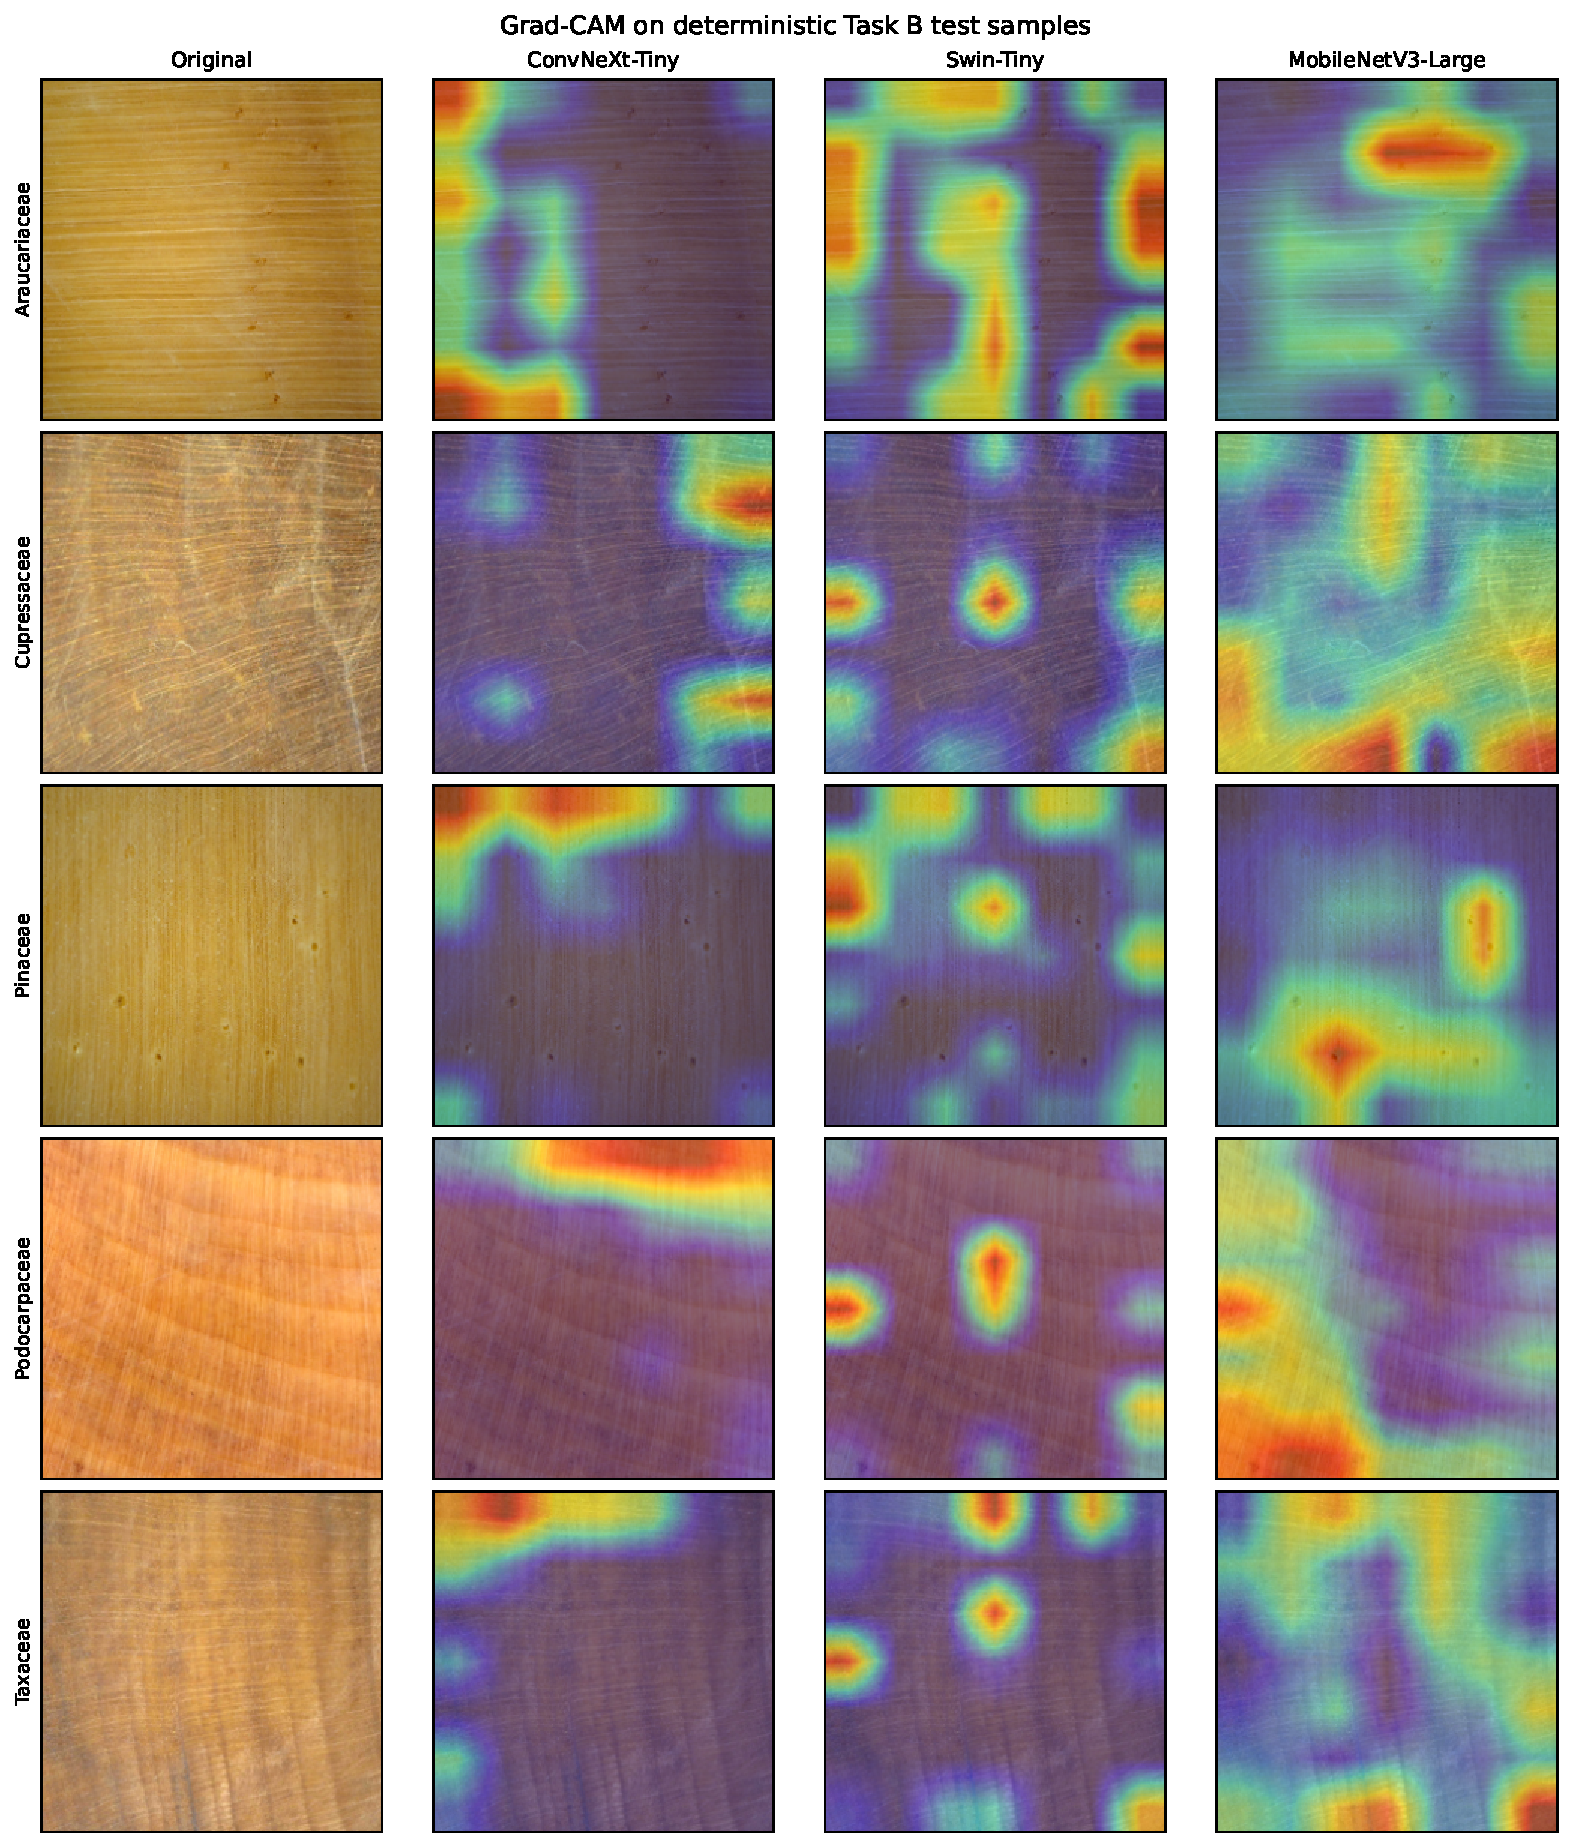
\includegraphics[width=\columnwidth]{artifact/person1/gradcam/fig_gradcam.pdf}
\caption{Bản đồ Grad-CAM cho ConvNeXt-Tiny, Swin-Tiny và MobileNetV3-Large trên năm ảnh test Task~B, mỗi họ một ảnh: \textit{Araucaria araucana}, \textit{Calocedrus rupestris}, \textit{Pinus radiata}, \textit{Podocarpus pilgeri} và \textit{Taxus wallichiana}. Ảnh được chọn theo quy tắc cố định trước: trong số những ảnh cả ba mô hình đều phân loại đúng, lấy ảnh gần nhất với mức độ tin cậy trung vị của ConvNeXt-Tiny trong họ của nó, phá hòa bằng đường dẫn ảnh. Không ảnh nào được chọn vì heatmap trông đẹp. Mỗi bản đồ đều lấy từ checkpoint seed 42 của các lần chạy ở Bảng~\ref{tab:task_b}. Các vùng quy gán trải rộng và ba kiến trúc làm nổi bật những vùng khác nhau trên cùng một ảnh; Grad-CAM định vị nơi gradient tựa vào và tự nó không xác định được đặc trưng nào đang được sử dụng.}
\label{fig:gradcam}
\end{figure}


Các vùng quy gán (attribution) trải rộng và phân tán trên khắp khung ảnh chứ
không tập trung vào những mốc giải phẫu nhận dạng được, và ba kiến trúc làm
nổi bật những vùng khác nhau trên cùng một ảnh. Đọc cùng với các phép thăm dò
ở Mục~\ref{vi:sec:results:convergence}, đây đúng là điều ta chờ đợi nếu bằng
chứng quyết định là tín hiệu tần số thấp trải đều trên ảnh chứ không phải đặc
trưng giải phẫu cục bộ. Grad-CAM cho biết gradient tựa vào đâu. Tự nó không xác
định được đặc trưng nào đang được sử dụng, và ở đây không đưa ra bất kỳ
cách đọc giải phẫu nào cho các bản đồ này.

\paragraph{Không gian đặc trưng.} Hình~\ref{fig:tsne} nhúng đặc trưng 768 chiều
trước lớp logit của ConvNeXt-Tiny seed 42 cho cả 532 ảnh test, giảm chiều bằng
PCA xuống 50 rồi bằng t-SNE xuống hai, với perplexity 30 và seed ngẫu nhiên cố
định. Các loài tạo thành những cụm phần lớn tách biệt, phù hợp với ma trận
nhầm lẫn gần như đường chéo ở Hình~\ref{fig:confusion}. Cấu trúc đáng chú ý
cho việc diễn giải là quan hệ giữa \textit{Pinus krempfii} và \textit{Pinus
dalatensis}, cặp duy nhất còn tồn tại ở mô hình tốt nhất
(Mục~\ref{vi:sec:results:perspecies}).

% Figure: t-SNE of ConvNeXt-Tiny pre-logit features, Task B test split
% Source   : artifact/person1/tsne/  (repo ManifoldsTeam/WoodID, branch p1,
%            commit d39a3f6b2cc5942e1e718c0dca86e89b0d81eb4d; see SOURCE.txt)
% Run id   : taskB17__main__seed_42__convnext_tiny  (same registry as Table 1)
% Artifacts: features_convnext_seed42_test.npz, tsne_embedding.csv,
%            tsne_metadata.json
\begin{figure}[!htbp]
\centering
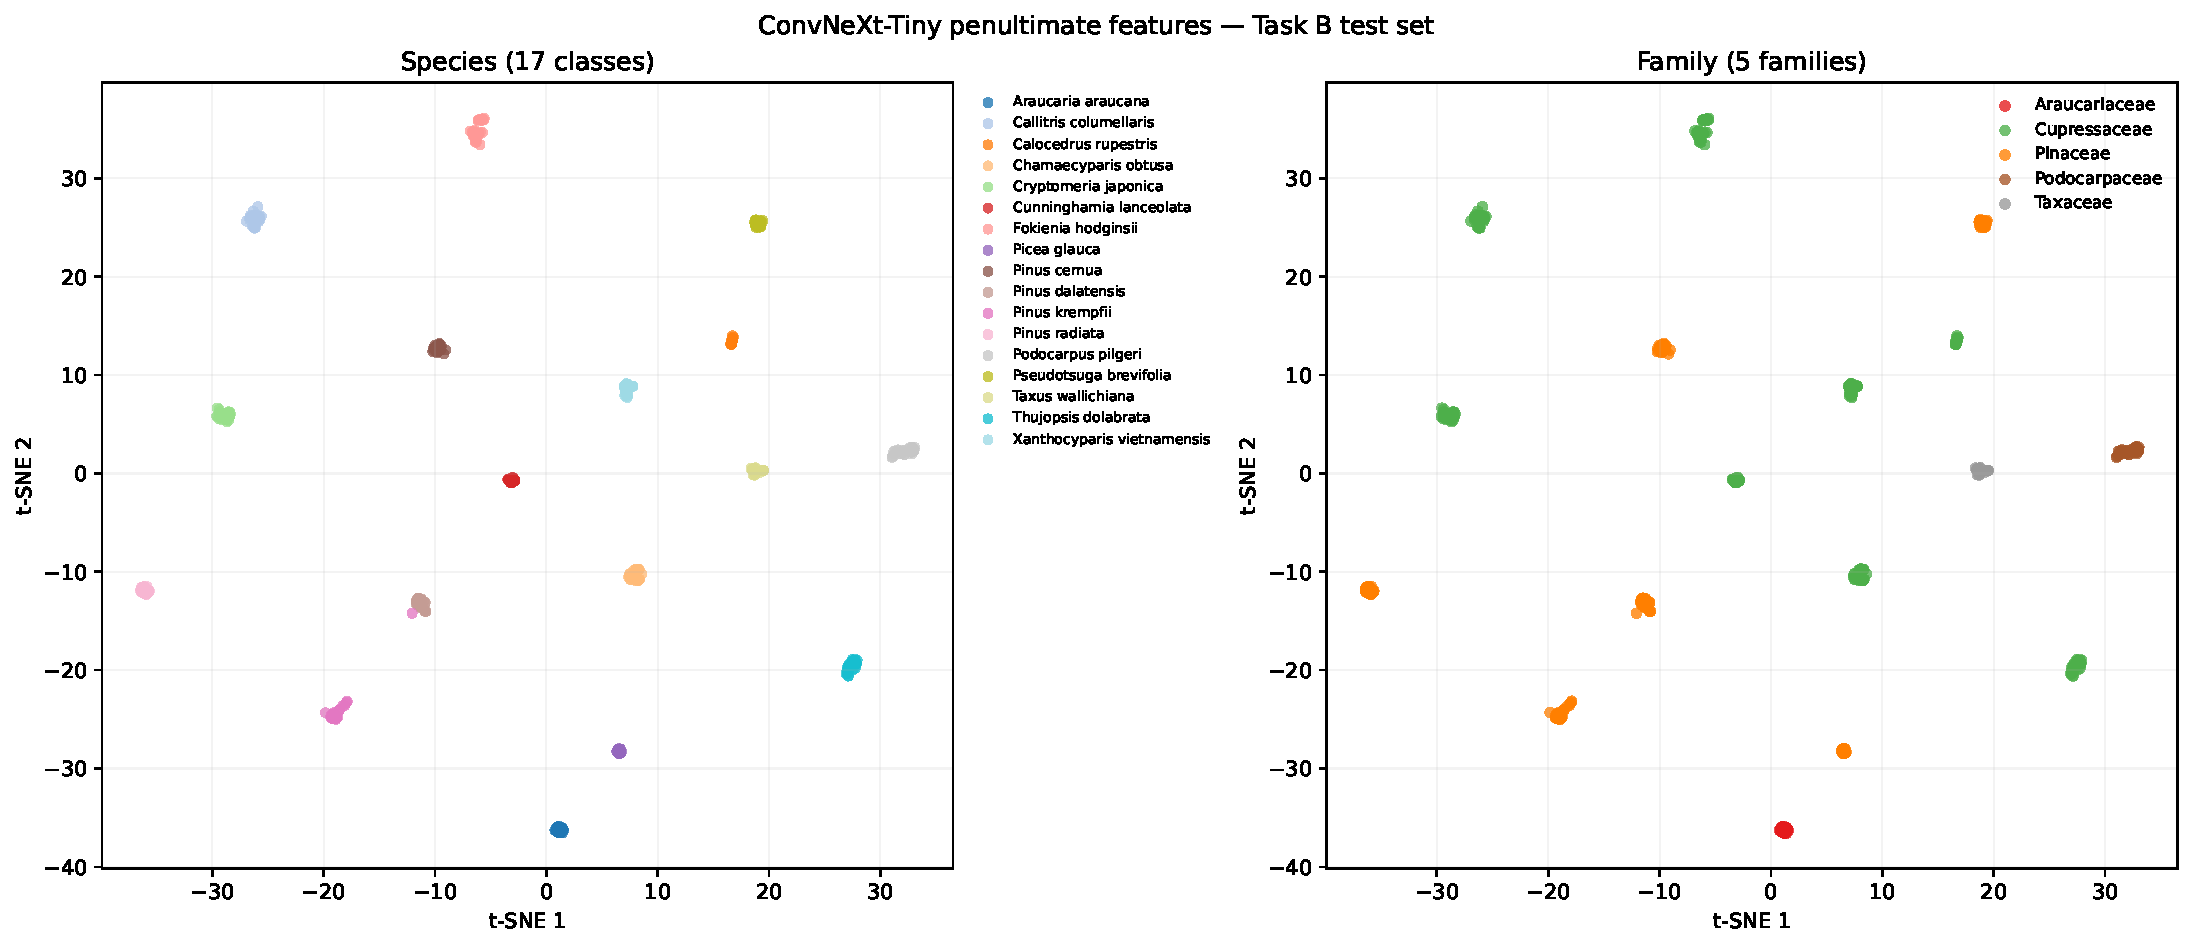
\includegraphics[width=\linewidth]{artifact/person1/tsne/fig_tsne.pdf}
\caption{Phép nhúng t-SNE hai chiều của đặc trưng ConvNeXt-Tiny cho cả 532 ảnh test Task~B, lấy từ lần chạy seed 42 ở Bảng~\ref{tab:task_b}. Đặc trưng là kích hoạt 768 chiều trước lớp logit, được chuẩn hóa, giảm xuống 50 chiều bằng PCA rồi xuống hai chiều bằng t-SNE với perplexity 30, khởi tạo PCA và seed ngẫu nhiên cố định. t-SNE chỉ bảo toàn láng giềng cục bộ: khoảng cách và diện tích cụm trong hình không phải metric, và phép nhúng được trình bày như một cách nhìn định tính về biểu diễn chứ không phải bằng chứng về tính tách được.}
\label{fig:tsne}
\end{figure}


Phép nhúng này là một phép chiếu được chọn để bảo toàn láng giềng cục bộ, và
khoảng cách trong đó không phải là metric. Phép nhúng được đưa vào như một
cách nhìn định tính về biểu diễn, không phải làm bằng chứng về tính tách được.
